\begin{center}
  \Huge\bfseries
  Securely and Privately Verifiable Protests
\end{center}
\begin{center}
  \large
  Daniel Bosk $\bullet$ Sonja Buchegger $\bullet$ Sébastien Gambs
\end{center}
\vspace{1.5em}

\begin{columns}[t]

  \begin{column}{0.32\linewidth}

    \begin{blueblock}{Scenario: The crowd-counting problem}
      \begin{itemize}
        \item Alice organizes a protest against Eve's regime.
        \item Bob, Carol and others show up.
        \item We want to know how many showed up to support Alice's cause.
      \end{itemize}
    \end{blueblock}

    \begin{figure}
      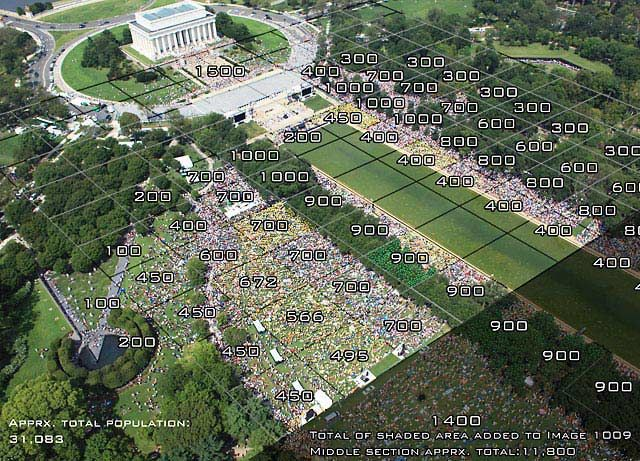
\includegraphics[width=0.9\linewidth]{fig/Jacobs-method.jpg}
      \caption{%
        Mostly used method, Jacob's method: divide the area into regions, 
        estimate the density in each region, sum them up.
      }
    \end{figure}

    \begin{orangeblock}{Computer vision methods}
      \begin{itemize}
        \item Computer vision does object recognition.
        \item Requires photos/video that cover the entire location, all the time.
        \item This will count people twice.
      \end{itemize}
    \end{orangeblock}

    \begin{orangeblock}{Other methods}
      \begin{itemize}
        \item Scan active mobile phones in the area.
        \item This requires some extra equipment.
        \item This catches bystanders who are not protesting.
      \end{itemize}
    \end{orangeblock}

    \begin{redblock}{Verifying protest participation}
      \begin{itemize}
        \item Alice organizes a protest against Eve's regime.
        \item Bob, Carol and others show up.
        \item {\color{olive!10!green!90} Alice wants to show that many support 
            her cause.}
        \item {\color{red} Eve wants to show that few support Alice's cause.}
        \item It's an adversarial setting!
        \item We need verifiable results.
      \end{itemize}
    \end{redblock}

    \begin{blueblock}{Requirements for verifiability}
      \begin{itemize}
        \item\label{EligibilityVerif} Eligibility: anyone can verify that each 
          participation proof provides temporal and spatial eligibility and that 
          it has not been counted before.

        \item\label{UniversalVerif} Universal verifiability: anyone can verify 
          that the result is according to the submitted participation proofs.

        \item\label{IndividualVerif} Individual verifiability: every participant 
          can verify that their participation proof is included in the global 
          count.
      \end{itemize}
    \end{blueblock}

    \begin{blueblock}{Requirements for privacy}
      \begin{itemize}
        \item The verifiability protocol should not increase the risk already 
          incurred by attending.
      \end{itemize}
    \end{blueblock}

    \begin{greenblock}{Our approach}
      \dots
    \end{greenblock}

  \end{column}

  \hfill

  \begin{column}{0.32\linewidth}

    \begin{blackblock}{Designated protest}
      \begin{itemize}
        \item A protest is identified by its cause, captured in a 
          manifesto.
        \item The hash of the manifesto provides an unpredictable identifier 
          (\(cid\) in figures).
        \item It's difficult to create a second manifesto that disagrees but 
          gets the same identifier.
      \end{itemize}
    \end{blackblock}

    \begin{blackblock}{Privacy-preserving linkability}
      \begin{itemize}
        \item We want linkability to prevent Sybil attacks.
        \item We also want privacy.
        \item We use techniques from anonymous credentials to create identifiers 
          (\(pid, wid\) in figures).
        \item The identifiers are random but unique per protest, i.e.\ depends 
          on \(cid\).
        \item The accompanying \ac{NIZK} proof prevents cheating (used during 
          verification).
      \end{itemize}
    \end{blackblock}

    \begin{blackblock}{Temporal eligibility}
      \begin{itemize}
        \item We use a blockchain for commitments, freshness.
        \item Freshness: a protester must include the head (hash value) of the 
          blockchain in their proof shares (\(t_s\) in figures).
        \item This value is difficult to guess and prevents preparing proofs too 
          long in advance.
        \item Commitments: when a proof share is prepared, it is committed to 
          the blockchain for timestamping.
      \end{itemize}
    \end{blackblock}

    \begin{blackblock}{Location proofs and spatial eligibility}
      \begin{itemize}
        \item Each proof must be bound to the location.
        \item This is done using witnesses.
        \item A witness runs a distance-bounding protocol to ensure proximity.
        \item If in proximity, the witness will issue a witness identifier and 
          signature (\(wid, wsig\)).
      \end{itemize}
    \end{blackblock}

    \begin{blueblock}{Verifying the participation count}
      \begin{enumerate}
        \item We must verify the eligibility of each proof, i.e.\ of all its 
          shares.
        \item We must count these valid proofs.
        \item Each protester must check that their proof is indeed registered so 
          that it can be counted.
      \end{enumerate}
    \end{blueblock}

\begin{blackblock}{Eligibility and universal verifiability}

Universal verifiability (\cref{UniversalVerif}) means that anyone should be able 
to count the valid proofs.
To do this we must be able to verify the eligibility of a proof (i.e.\ of all 
its shares) and then count it if valid.
To verify the eligibility of a proof share, we must verify that \(pid\), \(wid\) 
and \(wsig\) are not just randomly generated numbers but they actually depend on 
the keys \(k_P\) and \(k_W\) (as illustrated in \cref{fig:ProofFig}).
We will do this with \ac{NIZK} proofs.
We note that these proofs are not needed until the verification step after the 
protest.
Thus \(pid, wid, wsig\) can be used in the proof shares (and all computations 
above) whereas their respective \ac{NIZK} proof can be computed and published 
after the protest.

Alice must provide \iac{NIZK} proof showing that \(pid = PRF_{k_P}(id)\) and 
that she knows a signature by the identity authority on \(k_P\).
\dots
[Details of how to do this, or maybe that will be in \cref{BuildingBlocks}. See 
issue \#27 for discussion.]

In the same manner, each witness must also provide \iac{NIZK} proofs for \(wid = 
  PRF_{k_W}(pid)\) and \(wsig = PRF_{k_W}(wid, t_s, l)\) as well as that the 
witness knows a signature by the identity authority on \(k_W\).
With these \ac{NIZK} proofs anyone can verify the validity, i.e.\ the 
eligibility, of the proof shares and thus also count them.

\end{blackblock}

\begin{blackblock}{Individual verifiability and receipt freeness}

The purpose of individual verifiability (\cref{IndividualVerif}) is to prevent 
an adversary from dropping participation proofs.
Thus each protester must verify that their own proof is indeed included.
This can be accomplished as follows.
After Alice commited to her proof (share) in the blockchain, she stores the hash 
of the block.
At a later time, she can still verify that the block is indeed still there.
At this point, this hash value is the only thing she must store for individual 
verifiability.

More specifically, to achieve receipt freeness (\cref{ReceiptFreeness}) Alice 
must remove her secret PRF key, \(k_A\).
With this key Eve can verify that Alice has submitted a proof by computing 
\(pid'\gets PRF_{k_A}(cid)\) and compare \(pid = pid'\).

\end{blackblock}

  \end{column}

  \hfill

  \begin{column}{0.32\linewidth}

    \begin{figure}
      \centering
      \begin{tikzpicture}[%
        -Latex,
        item/.style={rectangle,draw},
        edge from parent/.style={},
        ]
        \tikzset{%
          %grow'=left,%
          %level distance=5em%
        }
        \node[item] (proof) {Proof share}
        child {%
          node[item] (pid) {$pid$}
          child {%
            node[item] (cid) {$cid$}
            child {%
              node[item] (manifesto) {Manifesto}
            }
          }
        }
        child {%
          node[item] (wid) {$wid$}
        }
        child {%
          node[item] (ts) {$t_s$}
        }
        child {%
          node[item] (l) {$l$}
        }
        child {%
          node[item] (wsig) {$wsig$}
        }
        ;

        \path[every node/.style={font=\small}]
        (pid) edge node [anchor=south east] {$\in$} (proof)
        (wid) edge node [anchor=east] {$\in$} (proof)
        (ts) edge node [anchor=east] {$\in$} (proof)
        (l) edge node [anchor=west] {$\in$} (proof)
        (wsig) edge node [anchor=south west] {$\in$} (proof)
        ;

        \path[every node/.style={font=\small}]
        (manifesto) edge node [anchor=east] {$H(\cdot)$} (cid)
        (cid) edge node [anchor=east] {$PRF_{k_P}(\cdot)$} (pid)
        (pid) edge[bend right] node [anchor=north west] {$PRF_{k_W}(\cdot)$} (wid)
        % wsig
        (l) edge[bend right] (wsig)
        (ts) edge[bend right] (wsig)
        (wid) edge[bend right] node [anchor=north west] {$PRF_{k_W}(\cdot, \cdot, 
          \cdot)$} (wsig)
        ;

      \end{tikzpicture}
      \caption{%
        Structure of a proof share.
        The protester \(P\)'s identifier \(pid\) is computed using the protester's 
        key \(k_P\).
        The witness \(W\)'s identifier \(wid\) is computed using the witness's key 
        \(k_W\).
        \(t_s\) is a time interval and \(l\) is the coordinates of an area.
        The protest (cause) identifier \(cid\) is the hash value of the manifesto.
      }%
      \label{fig:ProofFig}
    \end{figure}%

    \begin{figure}
      \centering
      \begin{minipage}{\linewidth}
        \begin{align*}
          O\to \text{all}\colon & \text{manifesto} \\
          P\colon & cid\gets H(\text{manifesto}), \\
          & pid\gets PRF_{k_P}(cid) \\
          P\to W\colon & pid \\
          W\leftrightarrow P\colon & \text{perform distance bounding} \\
          W\colon & wid\gets PRF_{k_W}(pid), \\
          & wsig\gets PRF_{k_W}(wid, t_s, l) \\
          W\to P\colon & (wid, t_s, l, wsig) \\
          W\to S\colon & H(pid, wid, t_s, l, wsig) \\
          P\to S\colon & H(pid, wid, t_s, l, wsig) \\
          W\to S\colon & (pid, wid, t_s, l, wsig),\\
          & NIZK(wid = PRF_{k_W}(pid), \\
            & wsig = PRF_{k_W}(wid, t_s, l), \\
            & \exists sign(k_W)) \\
          P\to S\colon & (pid, wid, t_s, l, wsig),\\
          & NIZK(pid = PRF_{k_P}(cid), \exists sign(k_P))
        \end{align*}
      \end{minipage}
      \caption{%
        An overview of message exchanges.
        The organizer \(O\) broadcasts the manifesto.
        \(P\), \(W\) and their computations are as in \cref{fig:ProofFig}.
        Finally, both \(P\) and \(W\) submits the proof share to the storage \(S\).
      }%
      \label{fig:ProtocolOverview}
    \end{figure}

    \begin{purpleblock}{Conclusions}
      \dots
    \end{purpleblock}

    \printbibliography[heading=none]

  \end{column}

\end{columns}

